\documentclass[adraft]{eptcs}
\usepackage[utf8]{inputenc}

\usepackage[toc,page]{appendix}

% Defines \FloatBarrier
% The "section" parameter makes floats stay in the section they are defined in.
\usepackage[section]{placeins}

\usepackage{graphicx}
\graphicspath{ {figures/} }
%\usepackage{listings}
\usepackage{eslistings}
\usepackage{parcolumns}
\usepackage{amsmath}
\usepackage{url}
\usepackage{breakurl}
\usepackage{todonotes}
\usepackage{amssymb}

\usepackage{tikz-timing}
\usepackage{svg}
\usepackage{calc}
\usepackage{amsmath}
\usepackage{subfig}

% glossary terms
\newcommand{\nrFUS}{MAX\_FUS}
\newcommand{\addrW}{FU\_ADDRESS\_W}
\newcommand{\dataW}{FU\_DATA\_W}
\newcommand{\bufSize}{BUF\_SIZE}
\newcommand{\bankAddrL}{MEM\_BANK\_ADDR\_LENGTH}
\newcommand{\memWordL}{MEM\_WORD\_LENGTH}


\renewcommand{\abstractname}{Abstract}

% Define Language
\lstdefinelanguage{SCAD}
{
  % list of keywords
  morekeywords={immediate, move, branch, jump},
  sensitive=false, % keywords are not case-sensitive
  morecomment=[l]{//}, % l is for line comment
  morecomment=[s]{/*}{*/}, % s is for start and end delimiter
  morestring=[b]" % defines that strings are enclosed in double quotes
}

%TODO: center listings
\lstset{language=SCAD,frame=L,style=ESStyle,tabsize=2,basicstyle=\small\ttfamily}
%\lstset{language=C,frame=L,style=ESStyle,tabsize=2,basicstyle=\small\ttfamily}
%\lstset{language=C,frame=L,basicstyle=\small\ttfamily,tabsize=2}
\lstset{numbersep=10pt}
\lstset{xleftmargin=5.0ex}
\lstset{numbers=left}
% Captions to the bottom
\lstset{captionpos=b}
\lstset{breaklines=false}

% Not used and has a tendency to break code.
\lstset{mathescape=false}

\newcommand{\ie}{i.~e.}
\newcommand{\Ie}{I.~e.}
\newcommand{\eg}{e.g.}
\newcommand{\Eg}{E.~g.}


\begin{document}
\begin{titlepage}
	\title{}
	\centering
	\includegraphics[width=0.75\textwidth]{TUKL_LOGO_FELD_LINKS_RGB}\par\vspace{1cm}
	{\Large Department of Computer Science \\ \it Embedded Systems Group \par}
	\vspace{1cm}
	{\Large Master Project\par}
	\vspace{1.5cm}
	{\huge\bfseries Implementation of SCAD processor \par}
	\vspace{2cm}
	{\Large Julius Roob \\ Mahircan G{\"u}l \\ Syed Maisum Haider \\ Subash Kannoth \par}
	\vfill
	supervised by\par
	\Large{Tripti Jain}
	\vfill
% Bottom of the page
	{\large \today\par}
\end{titlepage}

	%\maketitle \newpage
	\section{abstract}	
		\begin{abstract}
\begin{center}
    \textbf{Abstract}\linebreak[2]
\end{center}
 
Current processor architectures offer instruction-level parallelism by duplicating processing resources and handling both instruction and data distribution from a central controller. Although this scheme offers high throughput on non-dependent instructions, existence of central register file cripples the performance on data dependent workloads where several consecutive instructions contend for registers, which results in serialization of the machine code and stalls on controller. 

In this work, we implement \emph{Synchronous Control Asynchronous Dataflow (SCAD)\cite{time_pre_mod_comp}} architecture, where instructions are issued in order but data movement is handled by processing elements that are connected to each other via data network. Similar to out-of-order super scalar processors, SCAD architecture enforces dataflow order of instructions. However, fundamental difference is the decentralized hazard resolving mechanism, in which the controller does not halt issuing instructions as long as there are enough processing elements available. Instructions are issued in-order (synchronously), while operands and results are moved out-of-order (asynchronously). Data dependencies within a block of operations are resolved by a VLIW like mechanism without incurring register file contention. 
\end{abstract} \newpage
		\tableofcontents \newpage
	
		
		\section{Instruction Set Architecture}
		Like the Transport Triggered Architecture (TTA), the main feature of the SCAD machine instruction set is the move instruction.
		Moves happen from the output buffer of one Functional Unit (FU) to the input of another.
		Those moves have an order given by the program, and all parallel or out-of-order execution is done transparently by the hardware.
		
		While all operations are performed by moving data between functional units, some initial data is required, for example the addresses of where inputs and results are located in memory.
		Two possible means of getting that initial data to the functional units were considered in design.
		Those two were to either have dedicated FIFOs for inputs and outputs of the processor and program, or extend the ISA by instructions to load values for the data network.
		For the first approach, all constants that are required for a program to run have to be made available through one or more FIFOs or ROMs that outputs data into the data network when a corresponding move instruction is issued.
		The second, which is inspired by the bachelor thesis of Sebastian Schumb \cite{Schu15}, is to add at least one instruction to load immediate values.
		
		To make this design as simple to implement as possible, it was decided to have the control unit be part of the data network like the FUs, and both load immediate values into an output buffer, and take branch conditions from and input buffer. %This is explained further in Section \ref{?}\todo{Add Section reference}.
		
		So, aside from the mandatory move instruction, the ISA has instructions for loading immediate values, jumping to fixed addresses and branching.
		An overview of those instructions is given in Figure [1].%\ref{fig:instruction_table}.
		
		Example programs can be found in the Appendices \ref{app:simple} and \ref{app:fib}.
		
		
		\begin{figure}[!ht]
			\begin{center}
				\begin{tabular}{| l | p{8cm} |}
					\hline
					\textbf{instruction} & \textbf{semantics} \\ \hline
					move src, dest & Move data from an output buffer to an input buffer by sending this instruction to the corresponding functional units. Data move will asynchronous \\ \hline
					jump address & Set PC to address. \\ \hline
					immediate data & Place data into output buffer of control unit. \\ \hline
					branch address & A no-op when the first data in the input buffer is a 0, jump to address otherwise. Will wait for data to arrive when there is none. \\ \hline
				\end{tabular}
				\label{fig:instruction_table}
				\caption{SCAD Architecture Instructions}
			\end{center}
		\end{figure}


	\section{Control Unit}
		
		A simple synchronous Control Unit(CU) is implemented to provide synchronous control.
The role of the control unit is to fetch instructions from the instruction memory, and broadcast it to the Functional Units via the Move Instruction Bus (MIB). For this purpose the CU contains Instruction Fetch (IF), Program Counter(PC) and  CU to MIB blocks.

\begin{figure}[!h]

\includegraphics[scale=0.5]{CU_Sys.png}

\end{figure}


		In classical sense, the program counter maintains the counter for the instruction address.
In case of branch instructions, this counter receives a branch offset which is for relative addressing. Table \ref{table:pc_description} describes the input/output ports.		

	\begin{table}[!h]
		\begin{tabular}{| c| c | c | p{9cm} |}
			\hline
			\textbf{name} & \textbf{direction} & \textbf{type} &  \textbf{description}\\ \hline			
			active & input & STD\_LOGIC & Signal from Ctrl\_Mov\_Instr. The signal is used to stall			 program counter increment in case of stall.  \\ \hline
			taken & output & STD\_LOGIC & Signal shows whether branch has been taken or not.  \\ \hline
			branch\_offset & input & data\_word & Branch offset for pc if jump is taken.  \\ \hline			
			pc & output & data\_word & Instruction address.  \\ \hline
			
				
		\end{tabular}
		
		\caption{PC ports \label{table:pc_description}}
		\centering
	\end{table}

		As per the name, the instruction fetch block fetches instruction from an asynchronous instruction memory.The instructions are then sent to Ctrl\textunderscore Mov\textunderscore Instr. In case of a stall signal from Functional Units, the Instruction fetch does not fetch any new instructions or issue new instruction to the Ctrl\textunderscore Mov\textunderscore Instr.Table \ref{table:instrfetch} describes the input/output ports.
\begin{table}[!h]
	\begin{tabular}{| c| c| c| p{9cm} |}
	\hline
	\textbf{name} & \textbf{direction} & \textbf{type} &  \textbf{description}\\ \hline			
	read\_en & output &  STD\_LOGIC & Enable Signal for memory.\\  \hline
	mem\_addr & output &  data\_word & Address to Read from Memory.\\  \hline
	pc\_addr & input &  data\_word & Instruction Address from PC.\\  \hline		
	stall &  input &  STD\_LOGIC & Stall Signal.\\  \hline
	\end{tabular}
	\caption{Instruction Fetch ports \label{table:instrfetch}}
	\centering
\end{table}


		Ctrl\textunderscore Mov\textunderscore Instr block is responsible for broadcasting instructions via the Move Instruction Bus. Ctrl\_Mov\_Instr uses a 2 step commit mechanism to account for stalls generated by the functional units. 	Ctrl\_Mov\_MIB ensures the Control Unit is stalled if the source or target of the current instruction generate a stall. The Control Unit will be stalled until these stall signals do not drop. Table \ref{table:ctrlToMib} describes the input/output ports.
\begin{table}[!h]
	\begin{tabular}{| c| c| c| p{9cm} |}
	\hline
		\textbf{name} & \textbf{direction} & \textbf{type} &  \textbf{description.}\\ \hline		
		instruction\_input & input & instruction & Instruction word from Instruction Fetch.\\ \hline
		ctrl\_mib & output & mib\_ctrl\_out & Data packet from Control Unit to MIB.\\ \hline
		active  & output & std\_logic & Enable signal, connected to stalls of Control Unit components.\\ \hline
		valid\_IF & input & STD\_LOGIC & Signals new instruction from IF.\\ \hline
		dtn\_data\_in	 & input & data\_port\_sending & Branch conditions are redirected to Control Unit via this signal.\\ \hline
		dtn\_data\_out & output & data\_port\_sending & Immediate arguments are redirected to Control Unit via this signal.\\ \hline
		stall & input & mib\_status\_bus & signal description.\\ \hline
	\end{tabular}
	\caption{Instruction Fetch ports \label{table:ctrlToMib}}
	\centering		
\end{table}		


	
	\section{Move Instruction Bus}	
			To take into account both stalls of source and destination functional units, the control unit sends move instructions in two phases, both of which are indicated by a rising edge of the "valid" flag. First, with phase low, the functional units only check whether there is space in the corresponding input and output buffers.
When stalls are asserted, the control unit waits until the signals are dropped.When no functional unit of the current instruction stalls, the phase being high signals a "write".
\begin{figure}[!h]
\begin{center}
\begin{tikztimingtable}
src & Z18D{source address}Z \\
dest & Z18D{destination address}Z \\
phase & LLLLLLLLLLLLLLHHHHLL \\
valid & LLLHHHHHHHLLHHHHHHLL \\
src\_stalled & LLLLLLLLLLLLLLLLLLLL \\
dest\_stalled & LLLLLHHHHHLLLLLLLLLL \\
\end{tikztimingtable}
\caption{2-Phase Commit on Move Instruction Bus with Destination Stalling}
\end{center}
\end{figure}

		\subsection{MIB Controller}
			\section{MIB Controller}
	MIB controller is the bridge between control unit and FU network. It establishes communication for both control and status signals, where the former is routed from controller to target and latter is from target to controller, both unidirectionally. Table \ref{table:mib_description} describes input/output ports.  
	
	
	
	\begin{table}[htbp]
		\begin{tabular}{| l| l | l | p{9cm} |}
			\hline
			\textbf{name} & \textbf{direction} & \textbf{type} &  \textbf{description}\\ \hline
			ctrl & input & mib\_ctrl\_out & control packet from controller. \emph{dest.fu} signal is used to select target. ctrl signal is steered to destination port without modification. \\ \hline
			stat & output & mib\_stalls & status packet from target. \emph{dest.fu} signal of \emph{ctrl} determines the address of target in which its status to be read.  \\ \hline
			mib\_ctrl & output & mib\_ctrl\_bus & control signal group. Every FU in network is connected to the bus in ascending order of their addresses.   \\ \hline
			mib\_stat & input & mib\_status\_bus & status signal group. Status output of FUs in network is connected through corresponding signal   \\ \hline
			
		\end{tabular}
		
		\caption{MIB ports \label{table:mib_description}}
		\centering
	\end{table}
	 
	
	Assuming target address $N$, Figures \ref{fig:ctrl_to_target} and \ref{fig:status_from_target} illustrate control and status packet transfers from controller to target, and from target to controller, respectively. Since availability of both source and destination is checked by controller before performing control operations, packet is held at the bus for a cycle duration only. 
	
	\begin{figure}[!hbp]
	\centering
	\subfloat[Control packet to target] {
			\begin{tikztimingtable}[timing/lslope=0]
				clk & 14{C} \\
				ctrl.valid & 3L2H9L \\
				ctrl.dest & 3X8D{$N$}3X \\
				ctrl.phase & 3X8D{COMMIT}3X \\
				mib\_ctrl[$N$] & 5X2D{ctrl}7X \\
				mib\_ctrl.valid[$N$] & 5L2H7L \\
			\end{tikztimingtable}
			\label{fig:ctrl_to_target}
		}
			%\caption{Control packet to target}
			%\centering
%	\end{subfloat}
	\hfill
	\subfloat[Status packet from target] {
			\begin{tikztimingtable}[timing/lslope=0]
				clk & 14{C} \\
				ctrl.valid & 3L2H9L \\
				ctrl.dest & 3X8D{$N$}3X \\
				ctrl.phase & 3X8D{CHECK}3X \\
				mib\_stat[$N$] & 5X2D7X \\
			\end{tikztimingtable}
			\label{fig:status_from_target} 
		}
			%\caption{Status packet from target}
			%\centering
	
	\caption{Control and status packet transfer}
	\end{figure}
	
		Design is straightforward, consisting of $1\times\nrFUS$ de-multiplexer for controller to network routing and $\nrFUS\times 1$ multiplexer for opposite direction. Target functional unit is selected by destination address field of MIB control input, regardless of the operation type.  Due to lack of tri-state ic in FPGA fabric to be used, there is many-to-one relationship for status signals between functional units and control unit. Output of every unit is encoded in bus controller using destination address from control unit as line select. However, the opposite is not necessarily true, since a single line from controller for control packages can be snooped by functional units. For simplicity, we prefer using separate lines for control messages as well, by steering packet from controller to target line using destination address as line select. Bus snooping for control messages will be featured after validating main functionality. Figure \ref{fig:mib} shows structure of bus controller.
	\begin{figure}[htbp]
		\centering
		\def\svgscale{0.50}
		\section{MIB Controller}
	MIB controller is the bridge between control unit and FU network. It establishes communication for both control and status signals, where the former is routed from controller to target and latter is from target to controller, both unidirectionally. Table \ref{table:mib_description} describes input/output ports.  
	
	
	
	\begin{table}[htbp]
		\begin{tabular}{| l| l | l | p{9cm} |}
			\hline
			\textbf{name} & \textbf{direction} & \textbf{type} &  \textbf{description}\\ \hline
			ctrl & input & mib\_ctrl\_out & control packet from controller. \emph{dest.fu} signal is used to select target. ctrl signal is steered to destination port without modification. \\ \hline
			stat & output & mib\_stalls & status packet from target. \emph{dest.fu} signal of \emph{ctrl} determines the address of target in which its status to be read.  \\ \hline
			mib\_ctrl & output & mib\_ctrl\_bus & control signal group. Every FU in network is connected to the bus in ascending order of their addresses.   \\ \hline
			mib\_stat & input & mib\_status\_bus & status signal group. Status output of FUs in network is connected through corresponding signal   \\ \hline
			
		\end{tabular}
		
		\caption{MIB ports \label{table:mib_description}}
		\centering
	\end{table}
	 
	
	Assuming target address $N$, Figures \ref{fig:ctrl_to_target} and \ref{fig:status_from_target} illustrate control and status packet transfers from controller to target, and from target to controller, respectively. Since availability of both source and destination is checked by controller before performing control operations, packet is held at the bus for a cycle duration only. 
	
	\begin{figure}[!hbp]
	\centering
	\subfloat[Control packet to target] {
			\begin{tikztimingtable}[timing/lslope=0]
				clk & 14{C} \\
				ctrl.valid & 3L2H9L \\
				ctrl.dest & 3X8D{$N$}3X \\
				ctrl.phase & 3X8D{COMMIT}3X \\
				mib\_ctrl[$N$] & 5X2D{ctrl}7X \\
				mib\_ctrl.valid[$N$] & 5L2H7L \\
			\end{tikztimingtable}
			\label{fig:ctrl_to_target}
		}
			%\caption{Control packet to target}
			%\centering
%	\end{subfloat}
	\hfill
	\subfloat[Status packet from target] {
			\begin{tikztimingtable}[timing/lslope=0]
				clk & 14{C} \\
				ctrl.valid & 3L2H9L \\
				ctrl.dest & 3X8D{$N$}3X \\
				ctrl.phase & 3X8D{CHECK}3X \\
				mib\_stat[$N$] & 5X2D7X \\
			\end{tikztimingtable}
			\label{fig:status_from_target} 
		}
			%\caption{Status packet from target}
			%\centering
	
	\caption{Control and status packet transfer}
	\end{figure}
	
		Design is straightforward, consisting of $1\times\nrFUS$ de-multiplexer for controller to network routing and $\nrFUS\times 1$ multiplexer for opposite direction. Target functional unit is selected by destination address field of MIB control input, regardless of the operation type.  Due to lack of tri-state ic in FPGA fabric to be used, there is many-to-one relationship for status signals between functional units and control unit. Output of every unit is encoded in bus controller using destination address from control unit as line select. However, the opposite is not necessarily true, since a single line from controller for control packages can be snooped by functional units. For simplicity, we prefer using separate lines for control messages as well, by steering packet from controller to target line using destination address as line select. Bus snooping for control messages will be featured after validating main functionality. Figure \ref{fig:mib} shows structure of bus controller.
	\begin{figure}[htbp]
		\centering
		\def\svgscale{0.50}
		\section{MIB Controller}
	MIB controller is the bridge between control unit and FU network. It establishes communication for both control and status signals, where the former is routed from controller to target and latter is from target to controller, both unidirectionally. Table \ref{table:mib_description} describes input/output ports.  
	
	
	
	\begin{table}[htbp]
		\begin{tabular}{| l| l | l | p{9cm} |}
			\hline
			\textbf{name} & \textbf{direction} & \textbf{type} &  \textbf{description}\\ \hline
			ctrl & input & mib\_ctrl\_out & control packet from controller. \emph{dest.fu} signal is used to select target. ctrl signal is steered to destination port without modification. \\ \hline
			stat & output & mib\_stalls & status packet from target. \emph{dest.fu} signal of \emph{ctrl} determines the address of target in which its status to be read.  \\ \hline
			mib\_ctrl & output & mib\_ctrl\_bus & control signal group. Every FU in network is connected to the bus in ascending order of their addresses.   \\ \hline
			mib\_stat & input & mib\_status\_bus & status signal group. Status output of FUs in network is connected through corresponding signal   \\ \hline
			
		\end{tabular}
		
		\caption{MIB ports \label{table:mib_description}}
		\centering
	\end{table}
	 
	
	Assuming target address $N$, Figures \ref{fig:ctrl_to_target} and \ref{fig:status_from_target} illustrate control and status packet transfers from controller to target, and from target to controller, respectively. Since availability of both source and destination is checked by controller before performing control operations, packet is held at the bus for a cycle duration only. 
	
	\begin{figure}[!hbp]
	\centering
	\subfloat[Control packet to target] {
			\begin{tikztimingtable}[timing/lslope=0]
				clk & 14{C} \\
				ctrl.valid & 3L2H9L \\
				ctrl.dest & 3X8D{$N$}3X \\
				ctrl.phase & 3X8D{COMMIT}3X \\
				mib\_ctrl[$N$] & 5X2D{ctrl}7X \\
				mib\_ctrl.valid[$N$] & 5L2H7L \\
			\end{tikztimingtable}
			\label{fig:ctrl_to_target}
		}
			%\caption{Control packet to target}
			%\centering
%	\end{subfloat}
	\hfill
	\subfloat[Status packet from target] {
			\begin{tikztimingtable}[timing/lslope=0]
				clk & 14{C} \\
				ctrl.valid & 3L2H9L \\
				ctrl.dest & 3X8D{$N$}3X \\
				ctrl.phase & 3X8D{CHECK}3X \\
				mib\_stat[$N$] & 5X2D7X \\
			\end{tikztimingtable}
			\label{fig:status_from_target} 
		}
			%\caption{Status packet from target}
			%\centering
	
	\caption{Control and status packet transfer}
	\end{figure}
	
		Design is straightforward, consisting of $1\times\nrFUS$ de-multiplexer for controller to network routing and $\nrFUS\times 1$ multiplexer for opposite direction. Target functional unit is selected by destination address field of MIB control input, regardless of the operation type.  Due to lack of tri-state ic in FPGA fabric to be used, there is many-to-one relationship for status signals between functional units and control unit. Output of every unit is encoded in bus controller using destination address from control unit as line select. However, the opposite is not necessarily true, since a single line from controller for control packages can be snooped by functional units. For simplicity, we prefer using separate lines for control messages as well, by steering packet from controller to target line using destination address as line select. Bus snooping for control messages will be featured after validating main functionality. Figure \ref{fig:mib} shows structure of bus controller.
	\begin{figure}[htbp]
		\centering
		\def\svgscale{0.50}
		\input{figures/mib.pdf_tex}
		\caption{MIB structure}
		\label{fig:mib} 
	\end{figure}
		\caption{MIB structure}
		\label{fig:mib} 
	\end{figure}
		\caption{MIB structure}
		\label{fig:mib} 
	\end{figure}
	\newpage
	\section{Data Trasport Network(DTN)}
				
		
		The Data Trasport Network is the core part of the SCAD architecture. The 32 \textit{Fuction-Units} are identified by its physical address in the architecture which ranges from 0 to 31. Each \textit{Function-Unit} has output 
		that can send the \textit{Data-packets} to any other \textit{Function-Unit} in a given point of time. The \textit{Data-Packet} structure is shown in the Figure \ref{fig:Data_Packet}. The intention is to get all the \textit{Data-packets}
		deliverd to the corresponding target \textit{Function-Units} in minimum time, possibly constant time. A constant time means the time taken is deterministic. It can be several clock cycles and it will be the same for 
		any permutations of set if input addresses.
		
		A \textit{Cross-Bar} switch network is a possible solution with a gurantee of constant time delivery of \textit{Data Packets} to the target, but we have to compramise the resource consumption which makes it fairly complicated 
		for 32 \textit{Function-Units}. In other words the $32 X 32$ cross connection itself will consume a major part of the resources of the complete system, which is not efficient. Another possible solution for this is to use 
		memory mapped bus. But in this case, again it does not guarantee a constant time delivery to the \textit{Function-Units}, since there will be cases where we have to prioritize the \textit{Data-Packets} based in addresses possibly 
		by using an Arbeiter. 
		
		As a tradeoff between resource consumption and time to deliver a \textit{Data-Packet}, a {Bitonic Network} and a {Beneš Network} are indentified as good choices among many parallel sorting networks. 
		We implemented the DTN with a Bitonic as well as with a Beneš Network. A {Bitonic Network} sort any possible permutations in of input in constant time which makes it an excellent choice as a network router.
		Basically all the \textit{Fuction-Units} can be connected to each outputs of a \textit{Bitonic sorter} with respect to the physical address and thus {Bitonic sorter} acts network router. 
		Before going deep on the actual implementation we would like to give a short introduction about {Bitonic sorter}.

			\begin{figure}[!ht]
				%\begin{center}
				%    \begin{tabu} to 0.8\textwidth { | X[4] | X[6] |  X[4] | X[6] | X[4] | X[2] | }
				%    \hline
				%    \texttt{Valid bit \newline (1)} & \texttt{Target address\newline(5)} & \texttt{Source Address\newline(5)} & \texttt{Target buffer\newline(1)} & \texttt{Source Buffer\newline(1)} & \texttt{Data\newline(32)} \\
				%    \hline
				%    \end{tabu}
				%  \end{center}
				\includegraphics[width=\linewidth]{Data_Packet.png}
				\caption{Data Packet struture}
			\label{fig:Data_Packet}
			\end{figure}



		\subsection{Bitonic Network}
						    A Bitonic Sort\cite{bitonic_ref} is a comparison based parallel sorting algorithm. A random input sequence in first converted into a Bitonic sequence , which monotonically increases and then decreases thus the name Bitonic.
			    The rotations applied to a Bitonic sequence is also Bitonic.The random input is coversion to Bitonic sequence is achieved with a \textit{Bitonic-Splitter}.\newline
			    Let \[ 
				  S = \langle x_0,x_1,..x_{n-1}\rangle 
				\] be Bitonic sequence such that
				\[
				    x_0 \leq x_1 \leq ... \leq x_{n/2-1} \quad \textrm{and} \quad  x_{n/2} \leq x_{n/2+1} \leq ... \leq x_{n-1}  \quad \textrm{holds}
				\]
			    Consider the following subsequences
				\[
				  S_{1} =  \langle min(x_0,x_{n/2}), min(x_1,x_{n/2+1}),..,min(x_{n/2-1},x_{n-1})\rangle
				\]
				\[
				  S_{2} =  \langle max(x_0,x_{n/2}), max(x_1,x_{n/2+1}),..,max(x_{n/2-1},x_{n-1})\rangle
				\]
			    with the following property.
				\[
				  \forall _{x} \forall _{y}. x \in S_{1}  \wedge  y \in S_{2} \quad x < y
				\]
			    Both $S_{1}$ and $S_{2}$ are Bitonic. A sorted sequence is produced as a result of applying $S_{1}$ and $S_{2}$ recursively. The above procedure is called \textit{Bitonic Split}. Firstly \textit{Bitonic Split} is performed 
			    in the input random sequence which trasforms any given sequence to a Bitonic sequence which is then fed to the \textit{Bitonic Merge} network. The \textit{Bitonic Merge} converts the splitted sequence to sorted sequence.
			    sequence. A 16 input Bitonic sorter configuration is shown in the Figure \ref{fig:BitonicSorter16}. In our case we expand the same configuration to a 32 input sorter . The outputs $z_{0}$ to $z_{31}$  will
			    be connected to the corresponding \textit{Function-Units} with respect to the physical address.
				    \begin{figure}[!ht]
					      \includegraphics[width=\linewidth]{BitonicSorter16.png}
					    \caption{A 16 input BitonicNetwork}
				    \label{fig:BitonicSorter16}
				    \end{figure}
			    The arrow indicates a Comparator. The up-down arrow indicates an ascending comparator and the down-to up indicates a descending one. Both the comparator element configurations are shown in Figure \ref{fig:Comparators}. 
			    An N input Bitonic Network consists of $O(N.log_{2}(N)^{2})$ comparators and has a combinatorial depth of $O(log_{2}(N)^{2})$.
				    \begin{figure}[!ht]
					      \includegraphics[width=\linewidth]{Comparators.png}
					    \caption{Basic $2 x 2$ comparator elements of a Bitonic sorter}
				    \label{fig:Comparators}
				    \end{figure}
			\subsubsection{Bitonic Network as Network Router}
				  The Bitonic Network is only a sorting network, does not have enough intelligence to act it as a network router in practical cases. Everything works well when all \textit{Function-Units} 
				  are ready to send the \textit{Data-Packets} to its target. But this is not the case most of the times. Many \textit{Function-Units} can still be in a state where its outputs are not ready,
				  at the same time some of the \textit{Function-Units} are ready with their outputs. In this case Bitonic Network can fail in routing the \textit{Data-packets} to the right destinations because all
				  that are not ready can feed an unknown \textit{Target-Address}. Two solutions were identified as the following.
				  \subsubsection{Bitonic Network with additional Routers}
					      This is a proposed solution before realizing the Bitonic-Banyan \cite{batcher_banyan_ref}( Batcher's Banyan)  network. In this case the invalid \textit{Target-Address} problem is sorted
					      out by adding and two extra stages at the input and output of the Bitonic Sorter. At input we add an \textit{Address-Resolver} module for each comparators. In the architecture an invalid 
					      addresses\footnote{An invalid address here means when the a \textit{Function-Unit} has no outputs ready at a given point of time to send to another \textit{Function-Unit}, 
					      which can result in any address at the input of the DTN. The \textit{VALID} bit is asserted to a \textit{LOW} in every clock cycle by the \textit{Function-Unit} when not \textit{Data-Packets} are ready.}
					      is identified by a \textit{VALID} bit in the \textit{Data-Packet} (Figure \ref{fig:Data_Packet}). All \textit{Functional-Unit} writes a \textit{LOW} to the \textit{VALID} bit of its output packets in every clock cycle unless an packet is ready. 
					      In this way the network can interpret the validity of the \textit{Data-Packet} and act accordingly. The \textit{Address-Resolver} feeds the input of each comparator with a predefined hardcoded address according to the position of the comparator. 
					      Figure \ref{fig:Address_Resolver} shows a implementation of the \textit{Address-Resolver}.
					      \begin{figure}[!ht]
							\includegraphics[width=\linewidth]{Address_Resolver.png}
						      \caption{Address resolution}
					      \label{fig:Address_Resolver}
					      \end{figure}
					      The \textit{Address-Resovler} is a simple combinatorial multiplexer which switches the address based on the \textit{VALID} bit of address and is connected to all the $N$ comparators of input.
					      For an $N$ input Bitonic network the hardcoded address is defined as $N -1 + C$ , where $C$ is the position of the the comparator which ranges from $1$ to $N$. This ensures the 
					      comparators are fed with an addresses which is greater that $N -1$, which enables the sorter to work even if some of the inputs are invalid. In other words the \textit{Address-Resovler}
					      switches the input of the Bitonic network to  valid address at the instant when the \textit{VALID} bit is \textit{HIGH}. One  more problem that to be resolved
					      still is the sorted output sequence the network. The sorter will sort the \textit{Data-Packets} with all the hardcoded addresses positioned at last of the address sequence but still the actual addresses can
					      be routed into wrong destinations. For eg: If the input is an address sequence $\langle31,X_{1},X_{2},..,X_{31}\rangle$ (where $X_{i}$ indicates invalid address) which results in the sorted output sequence 
					      of $\langle31,32,33,..,63\rangle$. The routing is wrong since the $31$ is routed to target $0$. To resolve this we have to use a stage of sequencial routers at the output of the network.
					      
					      
					      The routers have forward and reverse routing path and \textit{Data-packet} is routed to either forward or reverse path based on the distance to the target. The distance to each destination is hardcoded 
					      in a routing table which enables faster decision making. The configuration is shown in Figure \ref{fig:RouterNetwork} .The drawback is a \textit{stall} signal is required
					      to stop the network to take new  \textit{Data-packets} until the old ones are delivered to the corresponding target  \textit{Function-Units}. The worst case time for a packet to reach the target
					      from the router network will be $N / 2$ .In other words in the worst case we have to stall network for $N/2$ clock cycles without doing anything useful in that time. The best
					      case would be when all the inputs are valid. Besides the circuit is sequencial and the \textit{stall} is active which degrades the DTN performance. This is because the \textit{stall} creates backpressure which
					      will be propegated to all the \textit{Function-Units} and the \textit{Control-Unit}.Also a router element is a complicated state machine which consumes considerable amount of resources when we have $32$ instances of the same. 
					      This fact lead us to use a Bitonic-Banyan\cite{batcher_banyan_ref} cascaded network which resolves this address permutation problem in constant time.
					      \begin{figure}[!ht]
							\includegraphics[width=\linewidth]{RouterNetwork.png}
						      \caption{Router Network}
					      \label{fig:RouterNetwork}
					      \end{figure}
				  \subsubsection{Bitonic-Banyan Network}
					      We utilize the self routing property of a Bitonic-Banyan\footnote{A Bitonic-Banyan cascaded network is called a Batcher-Banyan network in the reference paper\cite{batcher_banyan_ref}.
					      We call it as Bitonic-Banyan  network all over this paper to give an intuitive meaning how the network is constructed.} network \cite{batcher_banyan_ref} when the invalid 
					      \textit{Target-addresses} are found at the input. The configuration contains
					      a Bitonic Sorting Network cascaded with a Banyan routing network. As in the case of a Bitonic Network we use the $2 X 2$ switching element(comparator) but the connection state of this
					      element is determined by the destination tags of the input, in our case the \textit{Target address}. A Bitonic network is capable or realizing arbritary permutations of the inputs. 
					      But still the routing is not proper with invalid \textit{Data-packet} at the inputs. Here comes the use of Banyan network which can route the sorted outputs to appropriate
					      \textit{Target addresses}. As mentined before, special kind of modified switching elements are used which is quite differant from the configuration of normal Bitonic comparators.
					      The switching elements are added with some extra logic to route the larger target address \textit{Data-packets} to the direction pointed by the arrow. 
					      Figure \ref{fig:Batcher_Switches} depicts the switch configuration in different possible scenarios. 
					      
					      An $X$ indicates incomplete inputs. This switch basically moves all the $X$s from the input sequence to the bottom of the sequence.
					      Thus for any input sequence of Data-Packets with a set of  the invalid addresses $\{U_{0},U_{1},..,U_{r-1}\}$, the Bitonic network will produce an output sequence of $\langle A_{0},A_{1},..,A_{K},..,U,U,..,U \rangle$ , where
					      $ K = 32 - r -1$. Figure \ref{fig:Batcher_Switches} shows the modified switching element for the Bitonic network of the DTN. The \textit{Normal-Switch} is an ascending comparator which is shown in Figure \ref{fig:Comparators} and
					      the \textit{Modified-Switch} the one which is shown in Figure \ref{fig:Switching_Element}. which handles the invalid address situation.
					      \begin{figure}[!ht]
						      \includegraphics[width=\linewidth]{Batcher_Switches.png}
						      \caption{Modified switch handles different scenarios in Bitonic network}
					      \label{fig:Batcher_Switches}
					      \end{figure}
					      \begin{figure}[!ht]
						      \includegraphics[width=\linewidth]{Switching_Element.png}
						      \caption{Switching element of Bitonic network}
					      \label{fig:Switching_Element}
					      \end{figure}
					      \begin{figure}[!ht]
						      \includegraphics[width=\linewidth]{Banyan_Tree.png}
						      \caption{An 8 input Banyan network}
					      \label{fig:Banyan_Tree}
					      \end{figure}
					      The next stage is a Banyan Network which takes up the sorted sequences by the Bitonic network and route to the proper destination. 
					      
					      It is proven \cite{batcher_banyan_ref} that 
					      an Banyan network can completely route a sorted sequence when the incomplete inputs appear either at high end or low end of the list without any conflicts. We have already moved all the incomplete \textit{Data-Packets}
					      to the lower end of the sequence with the help of modified switch. An 8 input Banyan network configuraion is shown in Figure \ref{fig:Banyan_Tree}. We simply expand the same to 32.
					      The \textit{Data-Packets} in the Banyan network is based on the $i^{th}$ bit of the \textit{Target-Address}, where $i$ is the stage index. For an $N$ input Banyan network we have $log_{2}(N)$ 
					      stages and combinatorial circuit depth. A Banyan newtwork is collision free if the input sequences are sorted ascending
					      thus in our case gurantees the delivery of \textit{Data-Packets} at proper destination since the Bitonic network in the previous stage will already produce an acending sequence. In our case 
					      the sequence can also have invalid \textit{Data-Packets} which is in the tail of the sequence. Different scenarios in handling of incomplete input for a Banyan switch is shown in Figure \ref{fig:Banyan_Switches}.
					      A $X$ corresponds to incomplete inputs. The valid inputs are the bit position of the stage $i$ of the \textit{Target-Address}. Based on this bit the \textit{Data-packet} is routed up or down.
					      \begin{figure}[!ht]
						      \includegraphics[width=\linewidth]{Banyan_Switches.png}
						      \caption{Different scenarios in Banyan network switch }
					      \label{fig:Banyan_Switches}
					      \end{figure}
					      It has also verified with benchmarks \cite{sorting_network_on_fpgas} that for $N > 8$ the latency due to combinatorial depth of a Bitonic network is more that when it is piplelined. So we have implemented 5 stage pipleline 
					      for th Bitonic network and a 5 stage for the Banyan network.Altogether for the SCAD arhitecture the synchronous \textit{Bitonic-Banyan} version of DTN is shown in Figure \ref{fig:Batcher_Banyan_Combined}.
					      \begin{figure}[!ht]
						      \includegraphics[width=\linewidth]{Batcher_Banyan_Combined.png}
						      \caption{DTN of SCAD arhitecture with Bitonic-Banyan network}
					      \label{fig:Batcher_Banyan_Combined}
					      \end{figure}


			
		\FloatBarrier
		\subsection{Beneš Network}
			\begin{figure}[!ht]
	\centering
	\includegraphics[width=0.7\linewidth]{benes_network.pdf}
	\caption{The basic structure of a Beneš network}
	\label{fig:benes}
\end{figure}

The Beneš network is an extension of the Banyan network.
It solves the problem that a Banyan network is not able to produce all possible permutations by mirroring the Banyan network and connecting the two.
An example for a Beneš network with 8 inputs is given in Figure \ref{fig:benes}.

The two halves of the network are different in the routing procedure employed.
For the output half, the destination of a data packet defines the exact setting of every switch on its path, because there always is only one possible choice.
The input half is responsible for conflict avoidance, which has a significantly higher complexity due to the fact that it depends on all inputs of one column of the network.

\begin{figure}[!ht]
	\centering
	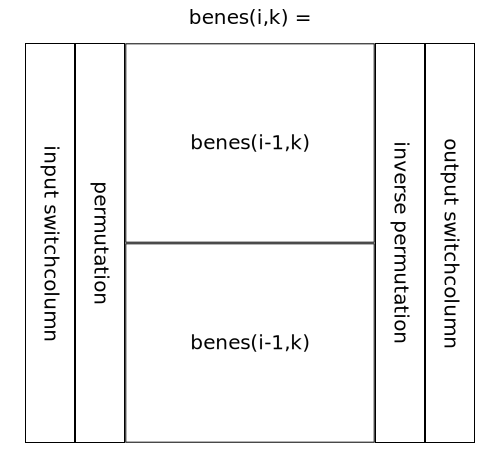
\includegraphics[width=0.7\linewidth]{benes_recursion.pdf}
	\caption{Recursive definition of a Beneš network}
	\label{fig:benes_recursion}
\end{figure}

For implementation, the recursive structure given in Figure \ref{fig:benes_recursion} was used.
A network with $2^n$ inputs is defined as $benes(n, n)$, where the first parameter gives the size of the specific network defined, and the second is used during recursion to remember the size of the whole network.

For this structure, the routing decision of the output switches is based on just bit $k - 1$, where a $0$ requires the packet to go up and $1$ to go down.

\begin{figure}[!ht]
	\centering
	\includegraphics[width=0.7\linewidth]{banyan_stall_switch.pdf}
	\caption{Structure of stalling banyan network switches}
	\label{fig:banyan_stall_switch}
\end{figure}

Together with the necessary registers for a pipelined network, the structure of those output switches is given in Figure \ref{fig:banyan_stall_switch}.
The second half of the Beneš network, the stalling Banyan, is built using only these switches, and requires only a minimal amount of logic (see Section \ref{sec:benes_resource_utilisation}) for a functionally complete DTN.

\begin{figure}[!ht]
	\centering
	\includegraphics[width=0.7\linewidth]{benes_companions.pdf}
	\caption{Paths of two outermost-layer companions}
	\label{fig:benes_companions}
\end{figure}

Causing more complexity, the routing decisions for the input switches of the Beneš network depend on all inputs of the network.
This is due to the fact that each pair of messages comes to an output switch has to arrive from two different subnetworks.
An example illustrating this is shown in Figure \ref{fig:benes_companions}.
Each destination address has a "companion", that is routed to the same output switch.

\begin{figure}[!ht]
	\centering
	\includegraphics[width=0.3\linewidth]{benes_input_column.pdf}
	\caption{Structur of Beneš network input switch column}
	\label{fig:benes_switchcolumn_in}
\end{figure}

\begin{figure}[!ht]
	\centering
	\includegraphics[width=0.8\linewidth]{benes_input_switch.pdf}
	\caption{Functional overview of Beneš input switch}
	\label{fig:benes_switch_in}
\end{figure}

To handle these dependencies properly, the input switch column of the recursive Beneš network uses reservation signals, where specific destinations are reserved by the switches sending packets to them so they are sent only once.
This is shown in Figure \ref{fig:benes_switchcolumn_in}, along with the lines for reservations from stalled packets, which need to have the highest priority because they can not be held back in the current architecture.
A detailed overview of an input switch is given in Figure \ref{fig:benes_switch_in}.

As a more simple solution, a lookup table for the first stage of a $32\times32$ Beneš network would require around $2.92\times10^{48}$ bytes.


\FloatBarrier
\subsubsection{Message Ordering}

		For each packet from source $s$ and destination $d$ and for the program order of move instructions $m_n(s_n, d_n) \prec m_{n+1}(s_{n+1}, d_{n+1})$, and delivery order of network $m_n \lhd m_k$, the following constraint has to hold:
	\begin{align*}
		& (m_n(s_n, d_n) \prec m_k(s_k, d_k)) \wedge (s_n = s_k \wedge d_n = d_k) \\
		& \Rightarrow (m_n(s_n, d_n) \lhd m_k(s_k, d_k))
	\end{align*}

	This is necessary since the input buffers cannot distinguish between different packets that have equal sources and destinations.
	
	With the recursive structure of the Beneš network and possible stalling at each input step, this constraint can not be guaranteed and is a case for which the network might work incorrectly.
	This does not apply to the Banyan part of the network, since relevant message pairs take the same path and do not overtake each other.
	
\subsubsection{Resource Utilisation of the Beneš Network}
	\label{sec:benes_resource_utilisation}
	\begin{table}[!ht]
		
		\begin{center}
			\begin{tabular}{l | c | c }
				\textbf{Site Type}  & \textbf{Benes(\%)}&\textbf{Stalling Banyan(\%)} \\
				\hline \hline
				Slice LUTs          & 51.23             & 13.86 \\
				\quad LUT as Logic  & 51.23             & 13.86 \\
				\quad LUT as Memory & 0.00              & 0.00  \\
				Slice Registers     & 12.28             & 06.61 \\
				\quad Register as Flip Flop & 12.28     & 06.61 \\
				\quad Register as Latch     & 0.00      & 0.00  \\
				F7 Muxes                    & 1.53      & 0.00  \\
				F8 Muxes                    & 0.63      & 0.00 \\
			\end{tabular}
		\end{center}
		\caption{Resource utilization of DTN with Benes network}
		\label{fig:benes_utilisation}
	\end{table}
	
	As shown in Table \ref{fig:benes_utilisation}, the Beneš network takes significantly more logic than all other DTNs.
	This, together with the high circuit depth required, make this implementation an unsuitable candidate for the SCAD architecture data network.
	
	The stalling banyan network may be considered for applications where a small DTN is required.

		\section{Buffers}
	Temporary data storage within functional units is implemented with buffers. Design of input and output buffers are un-identical; \textit{data packets} from DTN and \textit{reservations} from MIB, together forming an operand, has to be handled in input buffer whereas output buffer simply stores the results. 
	
	
	A reservation $r_i$ is represented by source field address of an MIB packet. Once an address is reserved, buffer snoops DTN for valid data packages $d_j$ and notifies operand availability if and only if $r_i = d_j.src$, \ie \hspace{1pt} source field of incoming data matches with reservation. Subscript for packets represent cycle of arrival.
	
	Reservations on input are performed with FIFO ordering for retaining actual sequence of operations; reservation $r_i$ is executed before $r_{i+1}$ where $i$ denotes arrival time, given that data is ready for the preceding reservation. Whenever data is available for a reservation, \textit{available} signal is asserted for FU to read the data from head of buffer.  
	 Next two sections explain input and output buffers in detail.
	
	\subsection{Input buffer}
	Input buffer forms an operand when DTN has valid data and its source address (routed from FU) matches with any of the reserved addresses inside buffer. Clearly, in every cycle a search needs to be performed amongst reserved addresses for $d_j$. For that purpose, two structures are used namely \textit{look-up-table (lut)} for searching and \textit{buffer (buf)} for operand storage. Figure \ref{fig:input_buffer} shows these components.
	
	\begin{figure}[htbp]
		\centering
		\def\svgwidth{\columnwidth}
		\input{figures/input_buffer.pdf_tex}
		\caption{Input buffer structure}
		\label{fig:input_buffer} 
	\end{figure}
	
	For managing the buffer, variables $head$, $tail$, and $num\_elements$ are used. $head$ points to first element of the buffer and is incremented when a read is performed. $tail$ points to last element and is incremented on every write. $num\_elements$ keeps track of number of elements in the buffer and is incremented or decremented in case of write and read respectively. Since buffer is single channel, these signals are not subject to concurrent updates. Input/output ports are described in \ref{table:in_buffer_description}.
	
	lut is an array of 2-tuple $(found, index)$ with size \nrFUS, where found is a 1-bit signal and index is a logic vector of size $log_2\bufSize$. For index $i$, \textit{found} states where address $i$ is reserved in  buffer. Source address of the MIB control packet is used as index to table for marking the corresponding entry in case of a reservation $r_i$ by marking lut[$r_i$] $(found=1,index=tail)$. For example, search for incoming DTN packet $d_j$ can be performed by checking $lut[d_j.src].found\stackrel{?}{=}1$. If found, $lut[d_j.src].index$ can be used for indexing the buffer.
	
	buffer is an array of  $(ready, address, data)$ with size \bufSize, where ready is a 1-bit signal, and address and data is logic vector of matching size. \textit{ready} is set whenever a data and address pair for a reservation gets available. In case of a reservation $r_i$, after marking $found$ in \textit{lut}, $buf[lut[r_i].index].address$ is set to $r_i$ without modifying $data$ ir $ready$ fields. Continuing with the previous example, arrival of data package with $d_j.src=r_i$ triggers modifying corresponding buffer entry as $buf[lut[d_j.src].index] = (ready=1, address= r_i, data= d_j.data)$.  
	
	Since FIFO ordering of reservation arrival is enforced, only $head$ of the buffer can be read in case it is ready. This means that ready entries superseded by a non-ready entry cannot be read and processesd by functional unit. Inspection and simulation of such cases has crucial importance for performance evaluation of the architecture.
	
	%ADD describe when MIB and DTN writes at same time
	
	\begin{table}[!htb]
		\begin{tabular}{| l| l | l | p{8cm} |}
			\hline
			\textbf{name} & \textbf{direction} & \textbf{type} &  \textbf{description}\\ \hline
			mib\_addr & input & logic\_vector(\addrW) & address to be reserved \\ \hline
			mib\_en & input & logic & enable strobe for address reservation \\ \hline
			dtn\_valid & input & logic & valid signal from DTN \\ \hline
			dtn\_data & input & logic\_vector(\dataW) & data from DTN \\ \hline
			dtn\_addr & input & logic\_vector(\addrW) & address from DTN \\ \hline
			fu\_read & input & logic & read enable from functional unit. Data at the buf[head] is written to the output when this signal is asserted \\ \hline
			available & output & logic & signals that an address/data pair is available at buf[head]. fu\_read is assumed to be set only when available is high \\ \hline
			full & output & logic & buffer full signal. Any reservation attempt on a non empty buffer is ignored \\ \hline
			empty & output & logic & buffer empty signal. This signal is obsolete and can be removed safely \\ \hline
			data\_out & output & logic\_vector(\dataW) & data output to functional unit. This signal is stable during a clock cycle after fu\_read is set \\ \hline
		\end{tabular}
		
		\caption{Input buffer ports \label{table:in_buffer_description}}
		\centering
	\end{table}
	
	\FloatBarrier
	\subsection{Output buffer}
	For storing results of operations inside FU, a single-channel FIFO buffer is used. It is a simple design that performs read/write and asserts empty/full. Every operation takes single cycle. Top-level scheme and port descriptions can be found in Figure \ref{fig:output_buffer} and Table \ref{table:out_buffer_description}, respectively.
	\begin{figure}[htbp]
		\centering
		\def\svgscale{0.5}
		\input{figures/fifo_buffer.pdf_tex}
		\caption{FIFO buffer structure}
		\label{fig:output_buffer} 
	\end{figure}
	
	\FloatBarrier
	
	\begin{table}[!htb]
		\begin{tabular}{| l| l | l | p{8cm} |}
			\hline
			\textbf{name} & \textbf{direction} & \textbf{type} &  \textbf{description}\\ \hline
			rw & input & logic & when low, data is read from buf[head], otherwise input is written to buf[tail]\\ \hline
			en & input & logic & enable strobe. rw is valid only when this signal is high \\ \hline
			data\_in & input & logic\_vector(\dataW) & data input from functional unit \\ \hline
			full & output & logic & buffer full signal. Writes are ignored when it is high \\ \hline
			empty & output & logic & buffer empty signal. When set, read operations cannot be performed on controlling functional unit. \\ \hline
			data\_out & output & logic\_vector(\dataW) & data output to functional unit \\ \hline
		\end{tabular}
		\label{table:out_buffer_description}
		\caption{FIFO buffer ports}
		\centering
	\end{table}
		\section{Functional Units(FU)}
	FUs are fundamental processing elements in this architecture. Connected to controller and rest of the units via MIB and DTN, each FU has the capability of storing operands/results and performing single operation. FUs are classified as \textit{Arithmetic-logic unit (ALU)} and \textit{memory}, depending on the type of processing performed. Next, design for both subsystems is explained.
	
	\begin{table}
		\begin{tabular}{| l| l | l | p{8cm} |}
			\hline
			\textbf{name} & \textbf{direction} & \textbf{type} &  \textbf{description}\\ \hline
			mib\_inp & input & mib\_ctrl\_out & control signal, including address to be reserved and target buffer index \\ \hline
			status & output & mib\_stalls & specifies whether input/output buffers are available for reservation. \\ \hline
			ack & input & logic & acknowledgment from interconnection network to indicate safe removal of current output entry from buffer \\ \hline
			dtn\_data\_in & input & data\_port\_sending & input from DTN \\ \hline
			dtn\_data\_out & output & data\_port\_sending & output to DTN \\ \hline
		\end{tabular}
		
		\caption{Input buffer ports \label{table:fu_alu_description}}
		\centering
	\end{table}
	\subsection{Arithmetical operations}
	Arithmetical operations take two operands and produce a single result. For that purpose, it consist of two input and one output buffers. As described in Table \ref{table:fu_alu_description}, \textit{index} field of \textit{mib\_inp} selects the input buffer to perform reservation. DTN input is directly connected to input buffers, since snooping capability is implemented within them.
	
	One of the features of SCAD architecture is the ease of plugging-in new operators without rigorous attempts for data-path modification. Hence, operation classes encapsulate the operators by using a well-defined interface. Either single-cycle, multi-cycle or pipelined, components implementing the interface can easily be hooked inside a FU, by only designing operator without making any effort on bus connections or buffer modification. Thus, we represent design of arithmetical functional units in two parts by first explaining generic interface and then top-level functional unit design.
	\begin{table}
		\begin{tabular}{| l| l | l | p{8cm} |}
			\hline
			\textbf{name} & \textbf{direction} & \textbf{type} &  \textbf{description}\\ \hline
			op1 & input & logic\_vector(\dataW) & operand from first buffer \\ \hline
			op2 & input & logic\_vector(\dataW) & operand from second buffer \\ \hline
			en & input & logic & when set, operation \textit{op} is performed using operands \\ \hline
			busy & output & logic & functional unit does not send new operands when unit is busy. Is useful only when operation to be performed requires stalling. Pipelined designs can be implemented by keeping it low   \\ \hline
			valid & output & logic & signals stable output value   \\ \hline
			res & output & logic\_vector(\dataW) & result of operation   \\ \hline
		\end{tabular}
		
		\caption{Input buffer ports \label{table:alu_description}}
		\centering
	\end{table}
	\subsubsection{Generic operation} \label{generic}
	
	Operator component of arithmetic FU uses ports defined in \ref{table:alu_description}. Control logic from FU sets \textit{en} signal when both buffers have their data available. When \textit{valid} is asserted, result of operation is written to \textit{res} for FU to read into its output buffer. Pipelined or multi-cycle designs can be realized by keeping \textit{en} and \textit{valid} signals high by changing operands in every cycle. FU considers stalls on both input and output buffers when driving \textit{en} signal. Anyways, only restriction is to prevent having \textit{valid} signal asserted when \textit{en} is low to avoid overflowing output buffer with stale results. Figure \ref{fig:alu} illustrated operator structure.
	
	Regardless of operation type (addition, multiplication, string comparison!), components adhering to the interface can simply be attached to the interconnection network. Abstracting functionality from architectural details results in easy additions to high-level instruction set. 
	
	\begin{figure}[htbp]
		\centering
		\def\svgscale{0.5}
		\input{figures/alu.pdf_tex}
		\caption{Arithmetic operator structure}
		\label{fig:alu} 
	\end{figure}
	
	\subsubsection{FU design}
	
	Although off-loading snooping logic to input buffers reduces complexity of FU, task of managing read/write signals amongst buffers causes non-negligible area cost in design. Main task performed by FU is to route the available operands from input buffers into operator and then write the result to output buffer.
	
	FU also checks incoming MIB packets' source address to decide if it should supply operands to the target FU. Assuming address $N$ for a FU, arrival of a MIB packet with $mib\_inp.src = N$ triggers an assemble phase where data at $head$ of output buffer $out\_buf$ is used for assembling a new DTN packet $d_j = (valid=1, src=N, dest=mib\_inp.dest, data=out\_buf[head])$ to be sent to destination via interconnection network. Even though it is not implemented in this version, FU should also check \textit{ack} signal coming from input of interconnection network and keep its output stable until it is asserted. Reason for such mechanism is the presence of DTN packets destined for same output, which are solved by adding FIFO buffers to the input of interconnection network for arbitrating access to same destination. In case when network buffer where FU is sending data through gets full, output should be held stable by FU until buffer has an empty space (until \textit{ack} is high), in which it is hard to derive an upper bound on number of cycles until arrival of acknowledgment. Due to the initial state of design and low probability of such event occurring, we simply discarded usage of \textit{ack} signal. Figure \ref{fig:fu_alu} shows top-level arithmetic FU.
	
	In the figure, red lines  belong to MIB, blue lines ones to DTN and yellow lines to internal data connections.
	As mentioned in \ref{generic}, FU waits for availability of data from both buffers. When available, a read is performed on both buffers. Then FU routes the operands to operator and waits for completion. Once done, result is written into output buffer.
	
	\begin{figure}[htbp]
		\centering
		\def\svgwidth{\columnwidth}
		\input{figures/fu_alu.pdf_tex}
		\caption{Arithmetic operator structure}
		\label{fig:fu_alu} 
	\end{figure}
	\subsection{Memory operations}
	Memory access is done via load/store functional units. For initial version, RAM is implemented using on-chip BRAM units, as an array of logic vectors, though it is not far from real design since caches should be introduced in some point anyways. Memory is divided into banks where each bank is shared by a pair of load/store units. This way, memory is simply segmented into regions and compiler/linker is responsible for translation from a flat address space to segmented addresses, since load/store units can access only to local RAM and bank. Figure \ref{fig:mem_top} shows an overview of subsystem.
	
	\begin{figure}[htbp]
		\centering
		\def\svgscale{0.5}
		\input{figures/memory_top.pdf_tex}
		\caption{Arithmetic operator structure}
		\label{fig:mem_top} 
	\end{figure}
	
	%Parameters defined in glossary section \ref{glossary_mem} represents size, %word-length and number of banks for memory system. Next, design of load and %store FUs are explained. Figures of MIB and DTN signals are omitted since they %are identical to those used in arithmetic FUs.
	\subsubsection{RAM}
	Main memory blocks are designed to infer synchronous read/write, dual-port, word-addressed RAM using BRAM blocks on fabric. With usage of acknowledgment signals for request, it resembles a synchronous master/slave bus protocol. Enable strobes for read/write are not driven directly by functional units, but via \textit{bank controller}, so RAM block does not check for conflicting read/write addresses. 
	
	Every access takes single cycle. Following read/write, respective acknowledgment signal is set to notify the functional unit. Table \ref{table:ram_description} includes detailed port definitions.
	 
	
	\begin{table}[htbp]
		\begin{tabular}{| l| l | l | p{7cm} |}
			\hline
			\textbf{name} & \textbf{direction} & \textbf{type} &  \textbf{description}\\ \hline
			re & input & logic & read enable strobe \\ \hline
			we & input & logic & write enable strobe \\ \hline
			r\_addr & input & logic\_vector(\bankAddrL) & address to read \\ \hline
			w\_addr & input & logic\_vector(\bankAddrL) & address to write \\ \hline
			data\_in & input & logic\_vector(\memWordL) & data to write \\ \hline
			r\_ack & output & logic & read acknowledgment signal. It is set when \textit{data\_out} is stable \\ \hline
			w\_ack & output & logic & write acknowledgment signal. Used for indicating write completion \\ \hline
			data\_out & output & logic\_vector(\memWordL) & data read from address \textit{r\_addr} \\ \hline
			
		\end{tabular}
		\caption{Input buffer ports \label{table:ram_description}}
		\centering
		\end{table}
	
	\subsubsection{Memory bank}
	A memory bank consists of a bank controller and a RAM unit. Load and store units cannot send commands to RAM module, but they request access from bank controller. This way, conflicts on read/write to same memory location at same cycle can be controlled. This module does not enforce any memory consistency model; only precaution is when a same address is to be accessed by multiple unit, store is given preference and load is stalled for one cycle. Otherwise, since memory is dual-channel reads/writes can be issued in same cycle.
	
	Even in presence of memory barrier instructions in high-level language, forcing a weak consistency model in rather \textit{chaotic} movement of data is a challenging task since order of memory accesses is not preserved despite having ordered reservations on FUs. 
	
	Data lines are not routed through bank but connected directly to RAM. Since there is no asynchronous read on memory, this does not cause any side-effects. Acknowledgment signals are directly connected to FUs as well. Port description can be found in Table \ref{table:bc_description}.
	
	\begin{table}[htbp]
		\begin{tabular}{| l| l | l | p{7cm} |}
			\hline
			\textbf{name} & \textbf{direction} & \textbf{type} &  \textbf{description}\\ \hline
			\multicolumn{4}{|c|}{\textit{FU Signals}} \\ \hline
			re & input & logic & read enable strobe from load FU \\ \hline
			we & input & logic & write enable strobe from store FU \\ \hline
			r\_addr & input & logic\_vector(\bankAddrL) & read address from load FU. Used for storing in register in case of conflicts  \\ \hline
			w\_addr & input & logic\_vector(\bankAddrL) & write address from store FU. Used for comparing with load address to check conflict  \\ \hline
			busy & output & logic & FUs do not send further requests when this signal is set \\ \hline
			\multicolumn{4}{|c|}{\textit{Memory signals}} \\ \hline
			re\_out & output & logic & read enable strobe to RAM \\ \hline
			we\_out & output & logic & write enable strobe to RAM \\ \hline
		\end{tabular}
		
		\caption{Input buffer ports \label{table:bc_description}}
		\centering
	\end{table}
	
	\FloatBarrier
	\subsubsection{Load/store unit}
	
	\paragraph{Load}
	Load unit has single input and single output buffer where input is used for storing memory address to be loaded and output is used for holding read data coming from memory. Table \ref{table:load_description} describes the input/output ports. Load unit has connections to both FU and bank controller where FU provides address to be read and load unit manages memory access transaction by setting commands to bank controller and checking acknowledgment from memory.
	\begin{table}[htbp]
		\begin{tabular}{| l| l | l | p{6cm} |}
			\hline
			\textbf{name} & \textbf{direction} & \textbf{type} &  \textbf{description}\\ \hline
			\multicolumn{4}{|c|}{\textit{FU Signals}} \\ \hline
			operand & input & logic\_vector(\bankAddrL) & operand from FU. Used as address on memory access \\ \hline
			busy & output & logic & indicates a memory transaction is on progress \\ \hline
			valid & output & logic & asserted when data loaded from memory is stable   \\ \hline
			res & output & logic\_vector(\memWordL) & output of memory access. Used by FU  \\ \hline
			\multicolumn{4}{|c|}{\textit{Memory signals}} \\ \hline
			res & input & logic\_vector(\memWordL) & output of memory access \\ \hline
			ack & input & logic & acknowledgement from memory. When set, \textit{res} is stable and can be read into internal register \\ \hline
			addr & output & logic\_vector(\bankAddrL) & address to load \\ \hline
			re & output & logic & read enable strobe to memory bank controller \\ \hline
		\end{tabular}
		
		\caption{Load unit ports \label{table:load_description}}
		\centering
	\end{table}
	
	
	\paragraph{Store}
	Store unit consists of two input buffers. Unlike other types of units, it does not have an output buffer, since store operation does not have output. Two inputs buffers are used for storing address/data pairs provided by DTN. Depending on the addressing modes, it is likely that address might be result of a computation, as well as an immediate from controller. Immediate operands are converted into DTN packets by control unit, so snooping DTN for write address works in both addressing modes.
	\begin{table}[htbp]
		\begin{tabular}{| l| l | l | p{6cm} |}
			\hline
			\textbf{name} & \textbf{direction} & \textbf{type} &  \textbf{description}\\ \hline
			\multicolumn{4}{|c|}{\textit{FU Signals}} \\ \hline
			fu\_address & input & logic\_vector(\bankAddrL) & address to write \\ \hline
			fu\_data & input & logic\_vector(\memWordL) & data to write \\ \hline
			busy & output & logic & indicates a memory transaction is on progress \\ \hline
			valid & output & logic & asserted when data loaded from memory is stable   \\ \hline
			\multicolumn{4}{|c|}{\textit{Memory signals}} \\ \hline
			ack & input & logic & acknowledgement from memory. Used for indicating write completion \\ \hline
			addr & output & logic\_vector(\bankAddrL) & address to load \\ \hline
			data & output & logic\_vector(\memWordL) & data to load \\ \hline
			we & output & logic & write enable strobe to memory bank controller \\ \hline
		\end{tabular}
		
		\caption{Store unit ports \label{table:store_description}}
		\centering
	\end{table}
	
	
	\subsubsection{FU design}
	Functional units encapsulating load and store components are similar to arithmetic FUs. Only difference is the number of input/output buffers and existence of connection between internal load/store units and RAM/bank controller components. Without MIB and DTN signals, load/store FUs are illustrated in Figure \ref{fig:load_fu} and Figure \ref{fig:store_fu}, respectively.
		\begin{figure}[htbp]
			\centering
			\def\svgscale{0.5}
			\input{figures/load_fu.pdf_tex}
			\def\svgscale{0.5}
			\caption{Load FU}
			\label{fig:load_fu} 
			\input{figures/store_fu.pdf_tex}
			\caption{Store FU}
			\label{fig:store_fu} 
		\end{figure}
	

	\section{Future Work}
	
	
		Having duplication as a separate functional unit may cause it to be a significant bottleneck.
		One feasible solution to this is the extension of the move instruction by an additional "non-destructive" move, where data sent is kept in the output buffer of the sender.
		
		
		Currently, load and store operations to same address in a given cycle is resolved by serializing the instructions such that write is given precedence over read. Evidently, this scheme does not provide any form of guarantees on memory access ordering.
		A future work is to enforce a memory consistency model, which can be implemented in memory bank controllers.
		
		%\todo[inline]{at least two more ideas}

	\newpage
	\section{Bibliography}
		\bibliographystyle{eptcs}
		\bibliography{references}
	\newpage
	
	\begin{appendices}
% 		\newpage
		\section{Memory Access and Branch}
			\label{app:simple}
			Basic example for memory access and branching:
			\lstinputlisting{assembler/simple.asm}
		
		\newpage
		\section{Fibonacci}
			\label{app:fib}
			\lstinputlisting{assembler/fibonacci.asm}
	\end{appendices}
	
\end{document}

